\documentclass[11pt,a4paper]{article}
\usepackage[utf8]{inputenc}
\usepackage[T1]{fontenc}
\usepackage{lmodern}
\usepackage[margin=2cm]{geometry}
\usepackage{amsmath,amssymb}
\usepackage{booktabs}
\usepackage{graphicx}
\usepackage{xcolor}
\usepackage{titlesec}
\usepackage{tabularx}
\usepackage{float}
\usepackage{hyperref}

\hypersetup{
    colorlinks=true,
    linkcolor=blue!70!black,
    citecolor=blue!70!black,
    urlcolor=blue!70!black
}

\titleformat{\section}{\large\bfseries}{\thesection.}{0.5em}{}
\titleformat{\subsection}{\normalsize\bfseries}{\thesubsection.}{0.5em}{}
\titlespacing*{\section}{0pt}{1.2ex plus 0.5ex minus .2ex}{0.6ex}
\titlespacing*{\subsection}{0pt}{1.0ex plus 0.4ex minus .2ex}{0.4ex}

\setlength{\parskip}{0.45em}
\setlength{\parindent}{0pt}

\begin{document}

\begin{center}
    {\LARGE \textbf{Projeto 3: VAE - \emph{Variational Autoencoder}}} \\[0.35em]
    {\large Disciplina: Introdução às Redes Neurais Artificiais} \\[0.3em]
    \textbf{Autor:} Vinícius Augusto Landim Andrade (RA: 169251) \\[0.2em]
    \textbf{Repositório / Código Reprodutível:} \url{https://github.com/vinicius-landim/neural-networks-course/tree/main/project-3-VAE}
\end{center}
\vspace{-0.5em}
\hrule
\vspace{0.8em}

% =====================================================================
\section{Configuração Experimental}

Este trabalho treina modelos generativos do tipo \textit{Variational Autoencoder}
(VAE) para o conjunto Fashion-MNIST e explora a organização do espaço latente
aprendido. Foram consideradas duas configurações de espaço latente, com
$2$ e $8$ dimensões, e, para cada uma, a topologia da rede foi escolhida pela
menor função de custo no conjunto de validação.

\subsection{Dados}

O Fashion-MNIST contém $70.000$ imagens em tons de cinza de $28 \times 28$ pixels,
divididas em dez classes de peças de vestuário e acessórios: camiseta, calça,
pulôver, vestido, casaco, sandália, camisa, tênis, bolsa e bota. Os pixels foram
normalizados para o intervalo $[0,1]$. As $60.000$ imagens de treino originais
foram separadas, de forma estratificada por classe, em $50.000$ para treino e
$10.000$ para validação. As $10.000$ imagens de teste foram usadas apenas na
avaliação final e na análise do espaço latente. Os rótulos não são usados no
treinamento, apenas na visualização e na análise.

\subsection{Modelo e função de custo}

O codificador recebe uma imagem $\mathbf{x}$ e produz os parâmetros de uma
distribuição normal no espaço latente, a média $\boldsymbol{\mu}$ e o logaritmo da
variância $\log \boldsymbol{\sigma}^2$, ambos com dimensão $d \in \{2, 8\}$. Um
ponto latente é amostrado pelo método de reparametrização,
\begin{equation}
  \mathbf{z} = \boldsymbol{\mu} + \boldsymbol{\sigma} \odot \boldsymbol{\zeta},
  \qquad \boldsymbol{\zeta} \sim \mathcal{N}(\mathbf{0}, \mathbf{I}),
\end{equation}
que mantém a amostragem derivável em relação a $\boldsymbol{\mu}$ e
$\boldsymbol{\sigma}$. O decodificador reconstrói a imagem $\hat{\mathbf{x}}$ a
partir de $\mathbf{z}$, com ativação sigmoide na saída para manter os pixels em
$[0,1]$. A função de custo, calculada por imagem, é a soma do erro de reconstrução
com a divergência de Kullback-Leibler entre a distribuição do codificador e a
distribuição a priori $\mathcal{N}(\mathbf{0}, \mathbf{I})$:
\begin{equation}
  \label{eq:loss}
  \mathcal{L} = \sum_{p=1}^{784} \left( x_p - \hat{x}_p \right)^2
  \; - \; \frac{1}{2} \sum_{j=1}^{d}
  \left( 1 + \log \sigma_j^2 - \mu_j^2 - \sigma_j^2 \right).
\end{equation}
O primeiro termo favorece reconstruções fiéis, e o segundo aproxima as
distribuições latentes de uma normal padrão, o que torna o espaço latente
contínuo e permite gerar novas imagens decodificando amostras
$\mathbf{z} \sim \mathcal{N}(\mathbf{0}, \mathbf{I})$.

\subsection{Arquiteturas e treinamento}

Foram comparadas três topologias para cada dimensão latente, resumidas na
Tabela~\ref{tab:arquiteturas}. Nas três, o decodificador espelha o codificador,
e as ativações intermediárias são ReLU. No caso da rede convolucional, ela reduz a resolução
pela metade a cada camada (\textit{stride} $2$) e usa convoluções transpostas no
decodificador para retornar a $28 \times 28$.

\begin{table}[H]
  \centering
  \small
  \begin{tabular}{lll}
    \toprule
    Modelo & Codificador (decodificador espelhado) & Parâmetros ($d=2$) \\
    \midrule
    MLP padrão    & $784 \to 256 \to d$ & $\approx 404$ mil \\
    MLP profunda  & $784 \to 512 \to 256 \to d$ & $\approx 1{,}07$ milhão \\
    Convolucional & Conv($32$) $\to$ Conv($64$) $\to$ Densa($256$) $\to d$ & $\approx 1{,}68$ milhão \\
    \bottomrule
  \end{tabular}
  \caption{Topologias candidatas. Na convolucional, cada camada usa
  \textit{kernel} $4 \times 4$ e \textit{stride} $2$
  ($28 \times 28 \to 14 \times 14 \to 7 \times 7$).}
  \label{tab:arquiteturas}
\end{table}

Os seis modelos foram treinados com os mesmos hiperparâmetros, apresentados na
Tabela~\ref{tab:config}. Cada modelo foi treinado por $50$ épocas, e foram
mantidos os pesos da época com menor perda de validação. A evolução das perdas, das reconstruções e das imagens geradas
foi acompanhada no TensorBoard.

\begin{table}[H]
  \centering
  \small
  \begin{tabular}{ll}
    \toprule
    Parâmetro & Valor \\
    \midrule
    Otimizador & Adam \\
    Taxa de aprendizado & $10^{-3}$ \\
    Tamanho do lote & $128$ \\
    Épocas & $50$ \\
    Seleção do modelo & época com menor perda de validação \\
    Semente aleatória & $42$ \\
    \bottomrule
  \end{tabular}
  \caption{Configuração do treinamento, comum a todos os modelos.}
  \label{tab:config}
\end{table}

\subsection{Análise do espaço latente}

A representação latente de cada imagem de teste é a média $\boldsymbol{\mu}$
produzida pelo codificador, sem amostragem. O espaço latente 2D é visualizado
diretamente, e o 8D é projetado em duas dimensões por Análise de Componentes
Principais (PCA). A variância explicada pela projeção é
$(\lambda_1 + \lambda_2)/\sum_j \lambda_j$, em que $\lambda_j$ são os autovalores
da matriz de covariância das representações.

Para quantificar a separação das
classes, foi usado o coeficiente de silhueta calculado com os rótulos reais, que
varia de $-1$ a $1$, sendo valores próximos de $1$ aqueles que indicam classes compactas e
separadas, os próximos de $0$ indicam classes encostadas ou sobrepostas, e valores
negativos indicam pontos mais próximos de outra classe do que da sua.

% =====================================================================
\section{Seleção da Topologia}

A Tabela~\ref{tab:selecao} apresenta a perda de validação de cada candidato e a
Figura~\ref{fig:curvas} mostra a sua evolução durante o treinamento. A MLP
profunda foi a melhor no espaço 2D e a rede convolucional no espaço 8D. Nas duas
dimensões, a MLP padrão teve a maior perda, o que indica que uma única camada
oculta limita a capacidade do modelo. Os dois modelos vencedores tiveram perdas
de teste praticamente iguais às de validação ($25{,}70$ e $22{,}99$), sem sinais
de sobreajuste.

\begin{table}[H]
  \centering
  \small
  \begin{tabular}{clcccc}
    \toprule
    $d$ & Modelo & Melhor época & \emph{Loss} total & Reconstrução & KL \\
    \midrule
    2
      & MLP padrão    & 49 & 27{,}62 & 22{,}50 & 5{,}12 \\
      & MLP profunda  & 50 & \textbf{25{,}68} & 20{,}47 & 5{,}21 \\
      & Convolucional & 49 & 26{,}13 & 20{,}78 & 5{,}35 \\
    \midrule
    8
      & MLP padrão    & 47 & 23{,}96 & 16{,}04 & 7{,}92 \\
      & MLP profunda  & 49 & 22{,}91 & 15{,}37 & 7{,}54 \\
      & Convolucional & 50 & \textbf{22{,}85} & 15{,}09 & 7{,}76 \\
    \bottomrule
  \end{tabular}
  \caption{\emph{Loss} no conjunto de validação (média por imagem) para cada
  topologia e dimensão latente. Em negrito, o modelo escolhido.}
  \label{tab:selecao}
\end{table}

\begin{figure}[H]
    \centering
    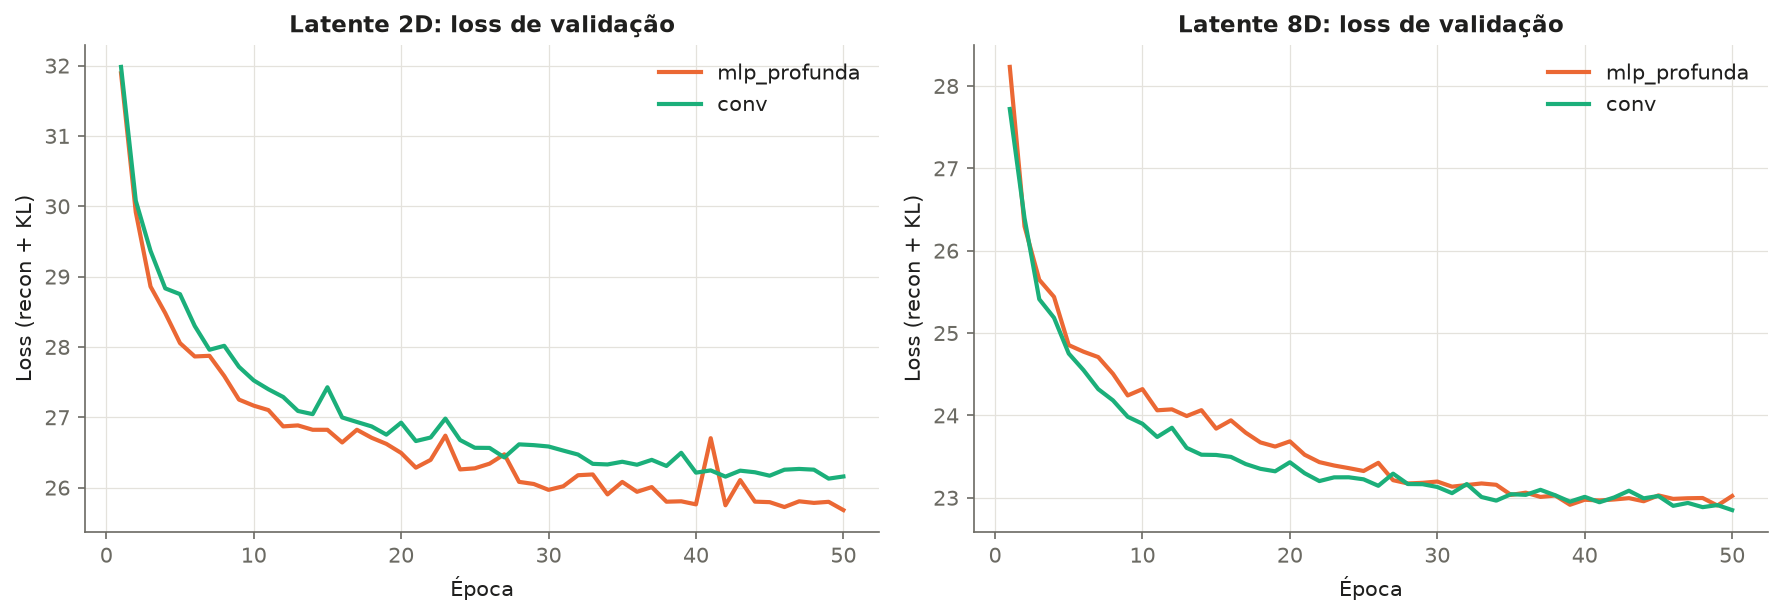
\includegraphics[width=\textwidth]{figs/curvas_validacao.png}
    \caption{Evolução da perda de validação durante o treinamento, para cada
    dimensão latente.}
    \label{fig:curvas}
\end{figure}

A diferença entre os dois melhores candidatos foi pequena ($0{,}45$ no espaço 2D
e $0{,}06$ no 8D) e cada modelo foi treinado uma única vez, então a ordem entre a
MLP profunda e a rede convolucional não é conclusiva. Além disso, os dois
vencedores atingiram o limite de $50$ épocas com a perda ainda em leve queda.

A comparação entre as dimensões mostra a relação entre os dois termos da
Equação~\ref{eq:loss}. Com $8$ dimensões, o erro de reconstrução foi cerca de
$26\%$ menor, enquanto o termo KL aumentou. O espaço maior permite guardar mais
informação sobre cada imagem, e o termo KL mede justamente essa quantidade de
informação. Por isso, a perda total só é comparável entre modelos com a mesma
dimensão latente.

% =====================================================================
\section{Reconstrução e Geração}

A Figura~\ref{fig:recon} compara uma imagem de cada classe do conjunto de teste
com as reconstruções dos dois modelos escolhidos. Observe que os dois preservam a silhueta e
o tom geral de cada peça, mas perdem os detalhes finos. Por exemplo, a estampa do pulôver e
as listras do casaco desaparecem, e as peças ficam com textura uniforme. No caso da
reconstrução com $8$ dimensões o resultado foi um pouco mais nítido; como na bota, que no
espaço 2D aparece mais clara e borrada. 

Note também a presença do desfoque, que é um comportamento característico do VAE com erro quadrático, pois quando o decodificador não consegue
distinguir entre variações parecidas, a saída que minimiza o erro é a média
entre elas.

\begin{figure}[H]
    \centering
    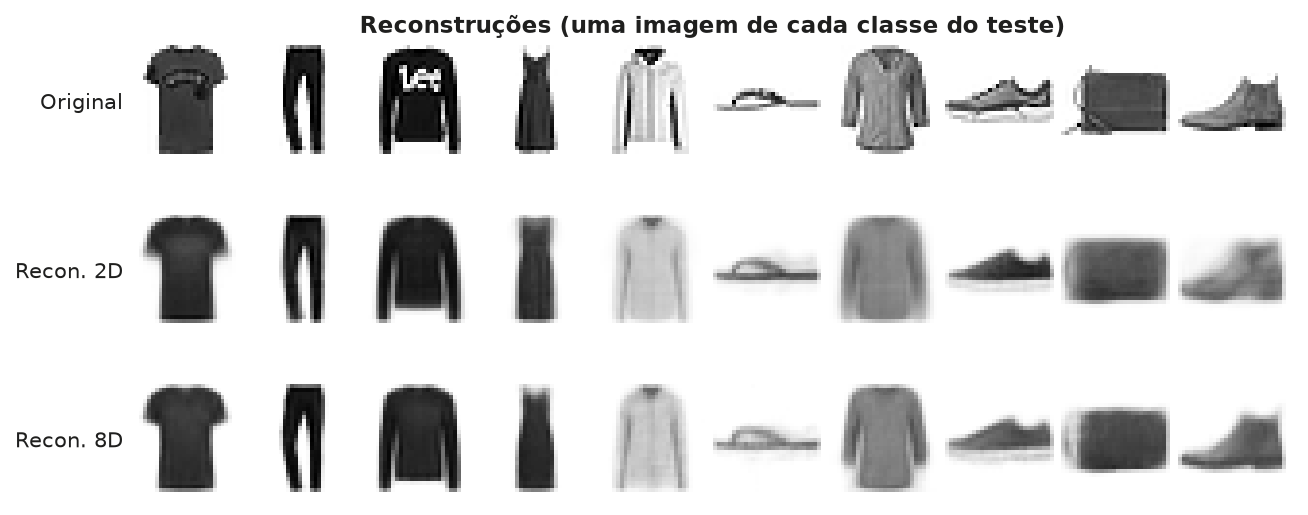
\includegraphics[width=0.9\textwidth]{figs/reconstrucoes.png}
    \caption{Imagens originais do conjunto de teste e reconstruções dos modelos
    escolhidos: MLP profunda (espaço latente 2D) e rede convolucional (espaço latente 8D).}
    \label{fig:recon}
\end{figure}

A Figura~\ref{fig:amostras} mostra imagens geradas a partir de pontos sorteados
da distribuição a priori. Nos dois modelos, a maior parte das amostras é uma peça
reconhecível, e todas as categorias aparecem, o que indica que o espaço latente
não tem grandes regiões sem significado. Algumas amostras, porém, são borradas ou
parecem combinar duas classes, como um tênis que se confunde com uma bota ou uma
camiseta com um vestido. Essas imagens correspondem a pontos nas regiões de
transição entre classes, que existem porque o espaço latente é contínuo.

\begin{figure}[H]
    \centering
    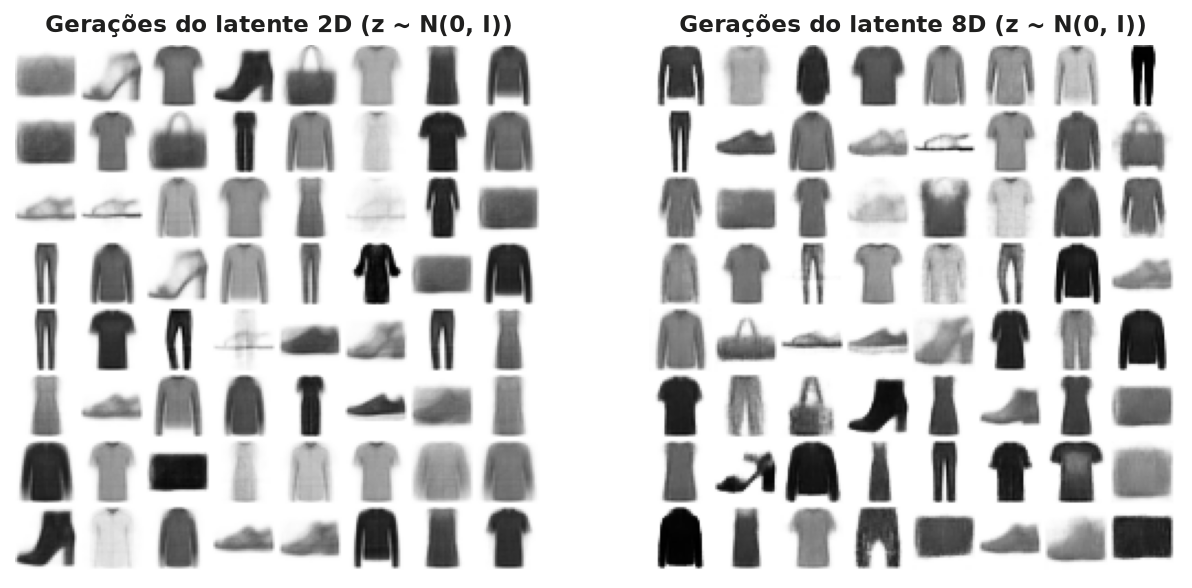
\includegraphics[width=0.9\textwidth]{figs/amostras.png}
    \caption{Imagens geradas a partir de $\mathbf{z} \sim \mathcal{N}(\mathbf{0},
    \mathbf{I})$ pelos modelos escolhidos: MLP profunda (espaço latente 2D) e
    rede convolucional (espaço latente 8D).}
    \label{fig:amostras}
\end{figure}

Um comportamente interessante que se pode obervar no acompanhamento pelo TensorBoard foi que, com os mesmos pontos latentes decodificados, nas primeiras épocas uma mesma amostra podia mudar
de categoria antes de se estabilizar. Isso ocorre porque o significado de cada
região do espaço latente não é fixo, já que o termo KL restringe apenas a distribuição
global dos pontos, e a posição de cada classe se reorganiza enquanto o modelo
aprende primeiro as diferenças mais gerais (por exemplo, calçados contra roupas)
e depois as mais finas.

% =====================================================================
\section{Espaço Latente 2D}

A Figura~\ref{fig:latente2d} mostra a representação latente das imagens de teste
no modelo 2D, e a Figura~\ref{fig:latente2d-classe} destaca cada classe em um
painel separado. Os pontos formam uma única nuvem contínua centrada na origem,
sem regiões vazias entre as classes, e as classes se distribuem como setores
radiais a partir do centro. Esse formato é consequência do termo KL, que puxa
todas as distribuições para perto da normal padrão.

\begin{figure}[H]
    \centering
    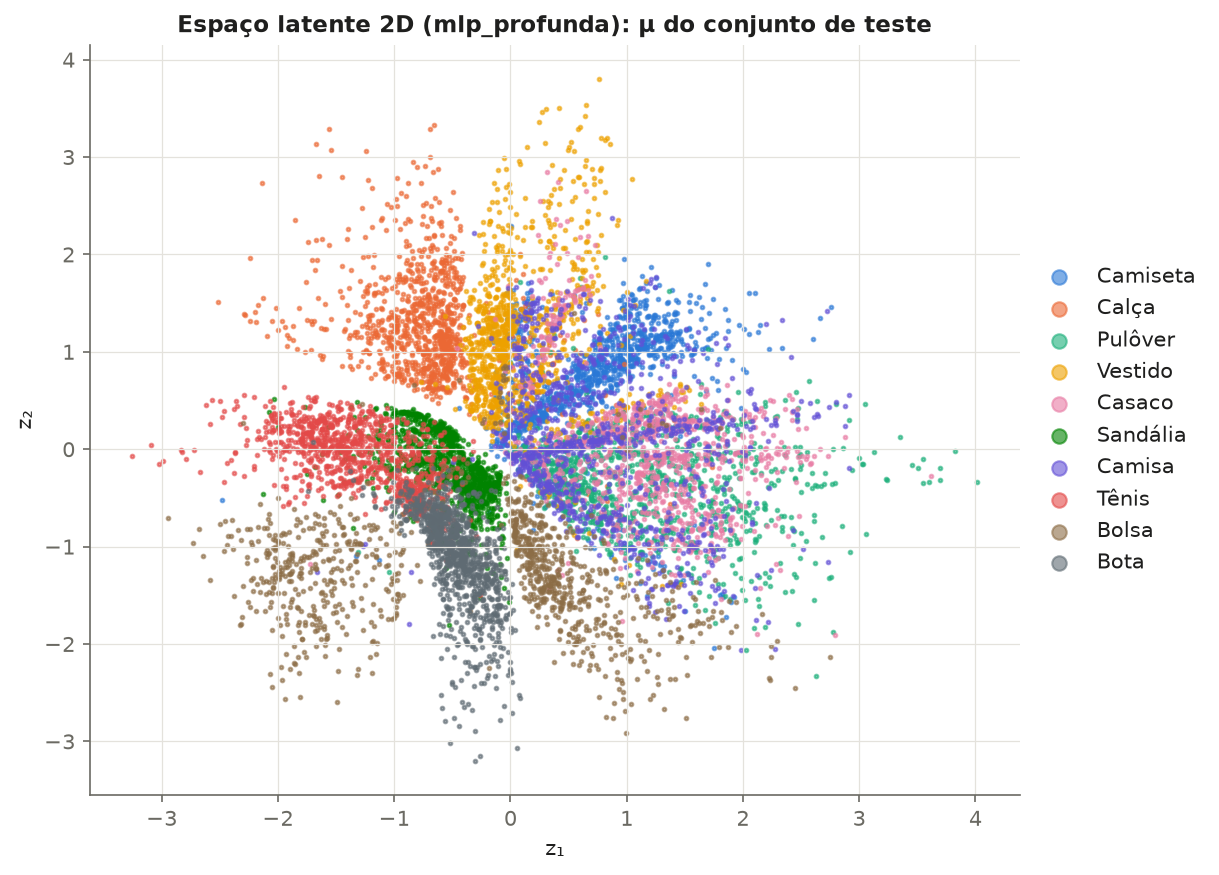
\includegraphics[width=0.75\textwidth]{figs/latente_2d.png}
    \caption{Espaço latente 2D (MLP profunda): média $\boldsymbol{\mu}$ de cada
    imagem do conjunto de teste, colorida pelo rótulo.}
    \label{fig:latente2d}
\end{figure}

\begin{figure}[H]
    \centering
    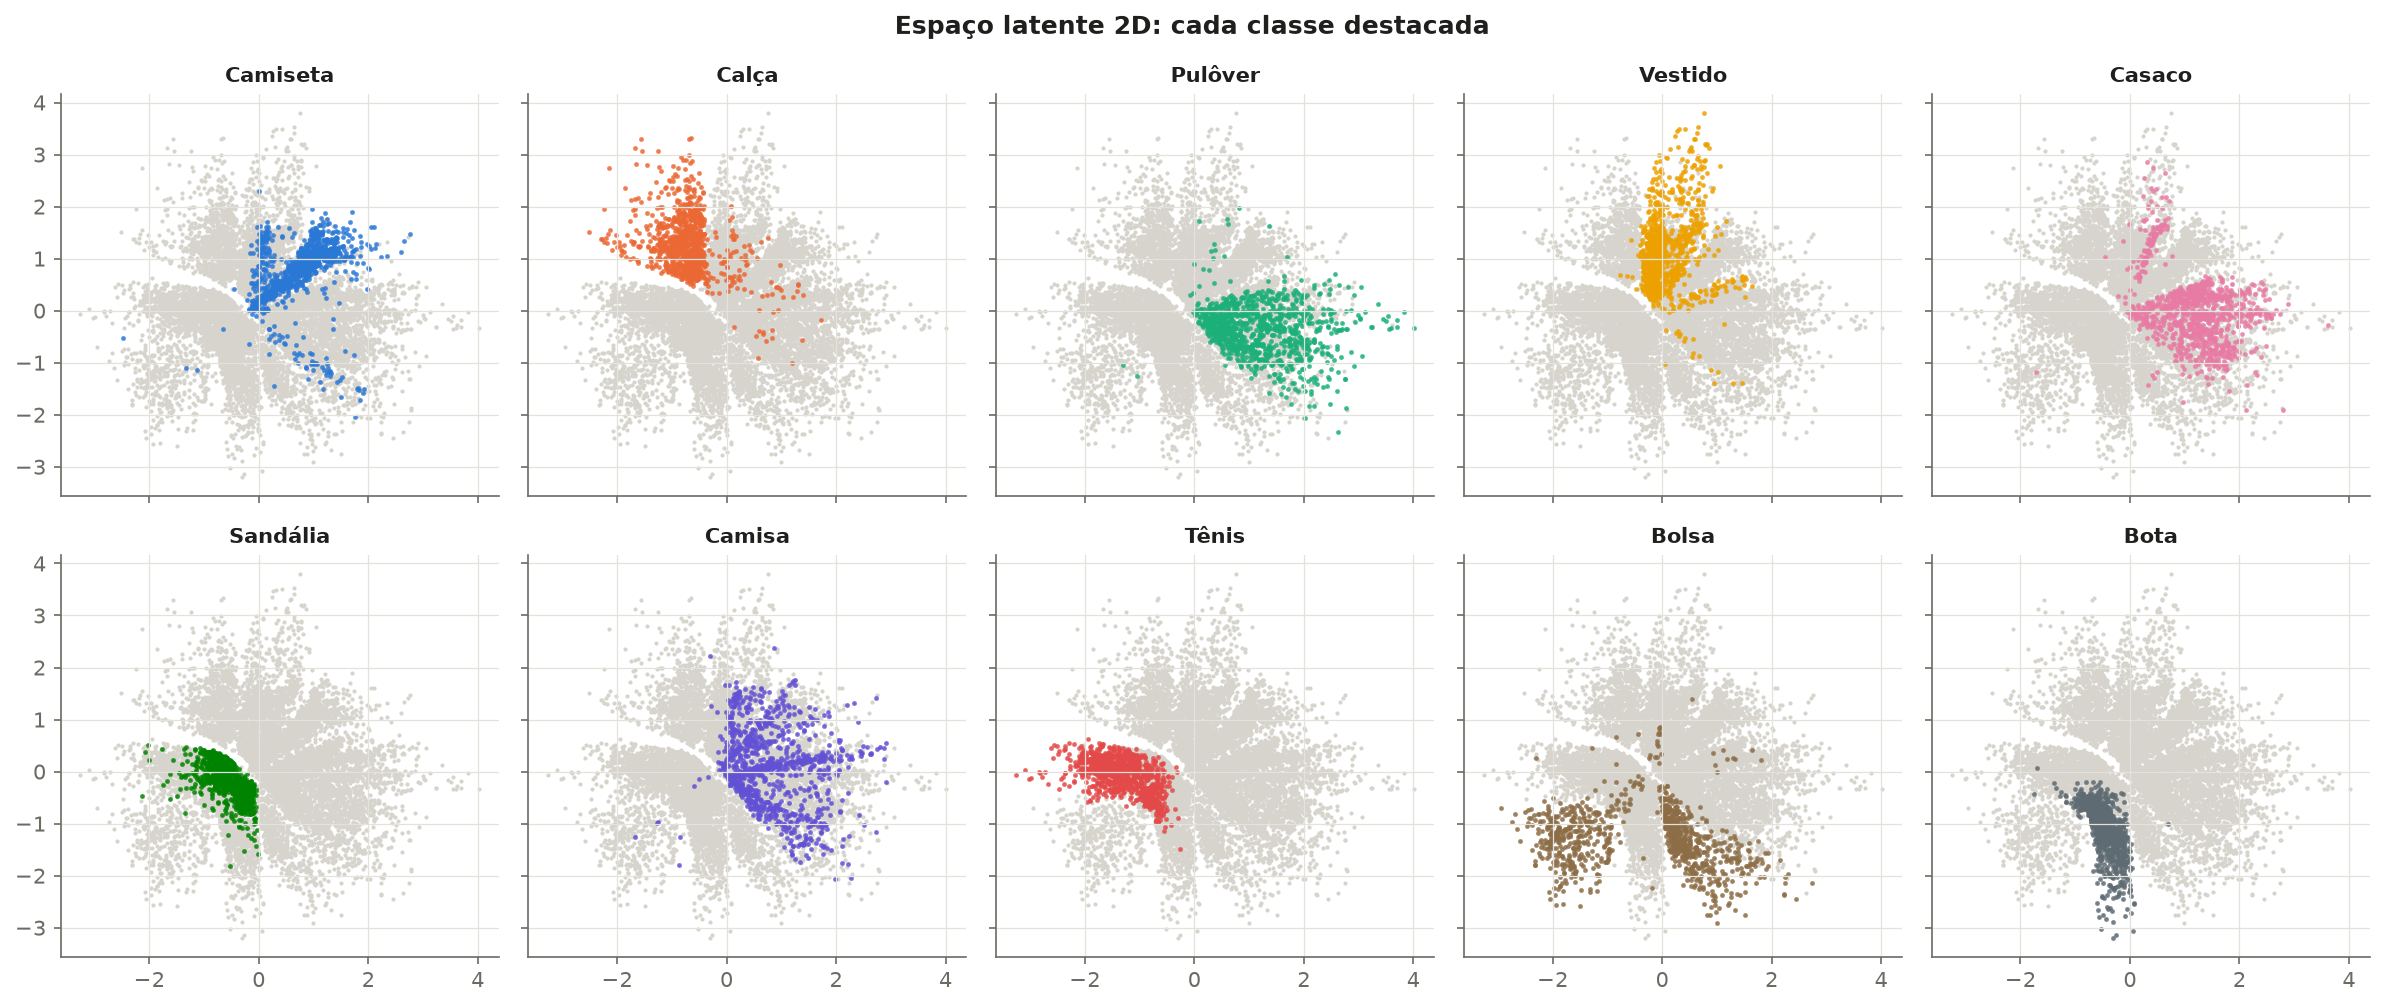
\includegraphics[width=\textwidth]{figs/latente_2d_por_classe.png}
    \caption{Espaço latente 2D com cada classe destacada sobre as demais.}
    \label{fig:latente2d-classe}
\end{figure}

Apesar de não terem sido usados no treinamento, os rótulos aparecem organizados
por semelhança visual. Com essa análise, é possível entender a concentração de pontos
que engloba cada classe e, principalmente, observar a aproximação de \emph{clusters}
entre classes com semelhança semântica.

Observe o caso dos três calçados (sandália, tênis e bota), em que eles ocupam setores
vizinhos e compactos à esquerda e abaixo da origem. O mesmo ocorre para as quatro peças de
vestimenta superior (camiseta, pulôver, casaco e camisa), que ocupam a mesma região e se
sobrepõem bastante, em especial a camisa, que se espalha sobre as outras três.
Em $28 \times 28$ pixels e sem cor, essas peças diferem apenas em detalhes como
o comprimento da manga e a presença de botões ou gola.

A bolsa é a única classe dividida em dois grupos separados, abaixo da origem.
O mapa da Figura~\ref{fig:manifold} indica a razão, que consiste no fato de que
um grupo corresponde a bolsas retangulares sem alça, e o outro a bolsas com alça. 
Ou seja, o modelo encontrou uma subdivisão da classe que os rótulos não registram.

\begin{figure}[H]
    \centering
    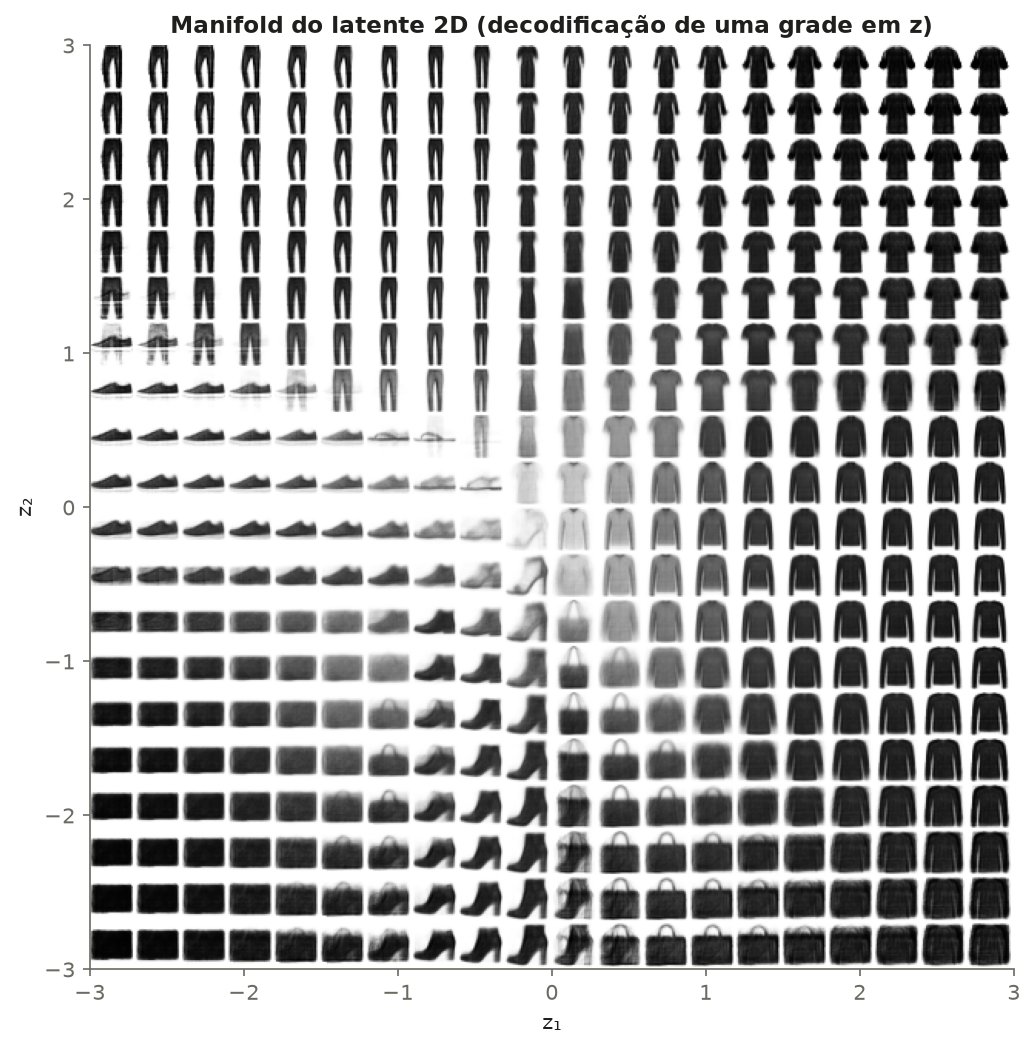
\includegraphics[width=0.7\textwidth]{figs/manifold_2d.png}
    \caption{Imagens decodificadas a partir de uma grade de pontos no espaço
    latente 2D, com $z_1, z_2 \in [-3, 3]$.}
    \label{fig:manifold}
\end{figure}

A Figura~\ref{fig:manifold} mostra o espaço latente pelo lado do decodificador.
As regiões do mapa correspondem às da Figura~\ref{fig:latente2d}: calças no
canto superior esquerdo, camisetas no superior direito, peças de manga longa à
direita, tênis à esquerda e bolsas e botas na parte inferior. As transições entre
regiões são graduais, como a calça que se estreita até virar vestido e depois se
alarga até virar camiseta, ou o tênis que ganha cano e salto até virar bota. Não
há regiões que decodifiquem em ruído, o que confirma que o espaço é contínuo.
Nas bordas da grade, que correspondem a pontos pouco prováveis pela distribuição
a priori, as imagens tendem a ficar mais escuras e exageradas.

% =====================================================================
\section{Espaço Latente 8D e Projeção por PCA}

A Figura~\ref{fig:pca-var} mostra a variância explicada por cada componente
principal das representações 8D. A projeção nas duas primeiras componentes
explica $45{,}6\%$ da variância. As cinco primeiras componentes têm autovalores
entre $0{,}65$ e $1{,}05$, e as três últimas têm variância praticamente nula.
Isso indica que três das oito dimensões latentes não foram usadas pelo modelo,
um fenômeno conhecido como colapso posterior, em que o codificador mantém essas
dimensões iguais à distribuição a priori para não pagar o custo do termo KL. Nas
dimensões usadas, os autovalores próximos de $1$ são esperados, pois o termo KL
aproxima cada dimensão de uma normal padrão. Como consequência, a variância fica
distribuída quase igualmente entre as componentes, e nenhuma projeção em duas
dimensões consegue representar a maior parte dela.

\begin{figure}[H]
    \centering
    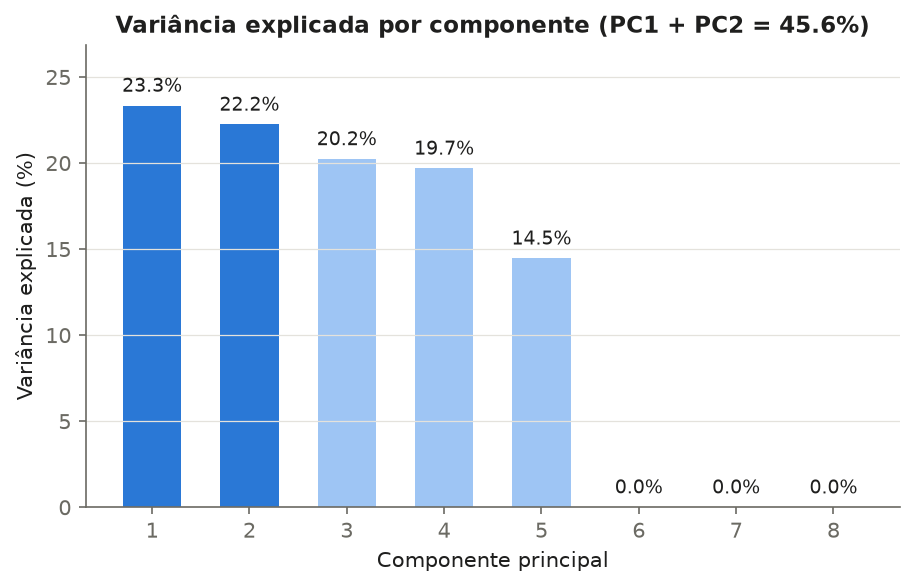
\includegraphics[width=0.6\textwidth]{figs/pca_variancia.png}
    \caption{Variância explicada por componente principal do espaço latente 8D.}
    \label{fig:pca-var}
\end{figure}

As Figuras~\ref{fig:pca8d} e~\ref{fig:pca8d-classe} mostram a projeção do espaço
8D. A estrutura é a mesma observada no espaço 2D: uma nuvem contínua, com os
calçados agrupados em uma região, a calça e o vestido em outra, a bolsa entre os
calçados e as peças de parte superior sobrepostas. Nesta projeção, a bolsa aparece
como um único grupo alongado, e a separação em dois estilos não é visível. As
mesmas relações de vizinhança surgiram nos dois modelos, com topologias e
dimensões diferentes, o que indica que elas refletem a semelhança visual entre as
peças, e não uma particularidade de um treinamento.

\begin{figure}[H]
    \centering
    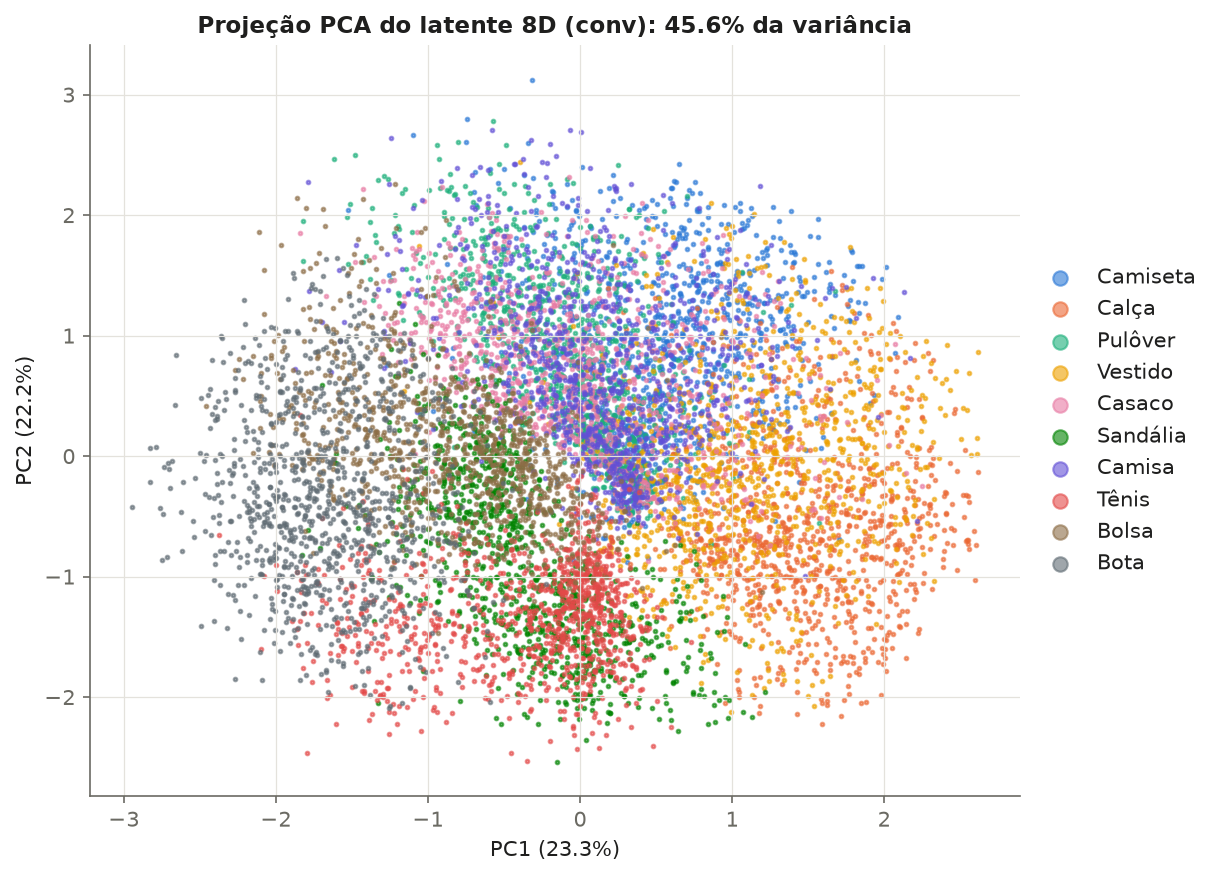
\includegraphics[width=0.75\textwidth]{figs/pca_8d.png}
    \caption{Projeção do espaço latente 8D (rede convolucional) nas duas
    primeiras componentes principais, colorida pelo rótulo.}
    \label{fig:pca8d}
\end{figure}

\begin{figure}[H]
    \centering
    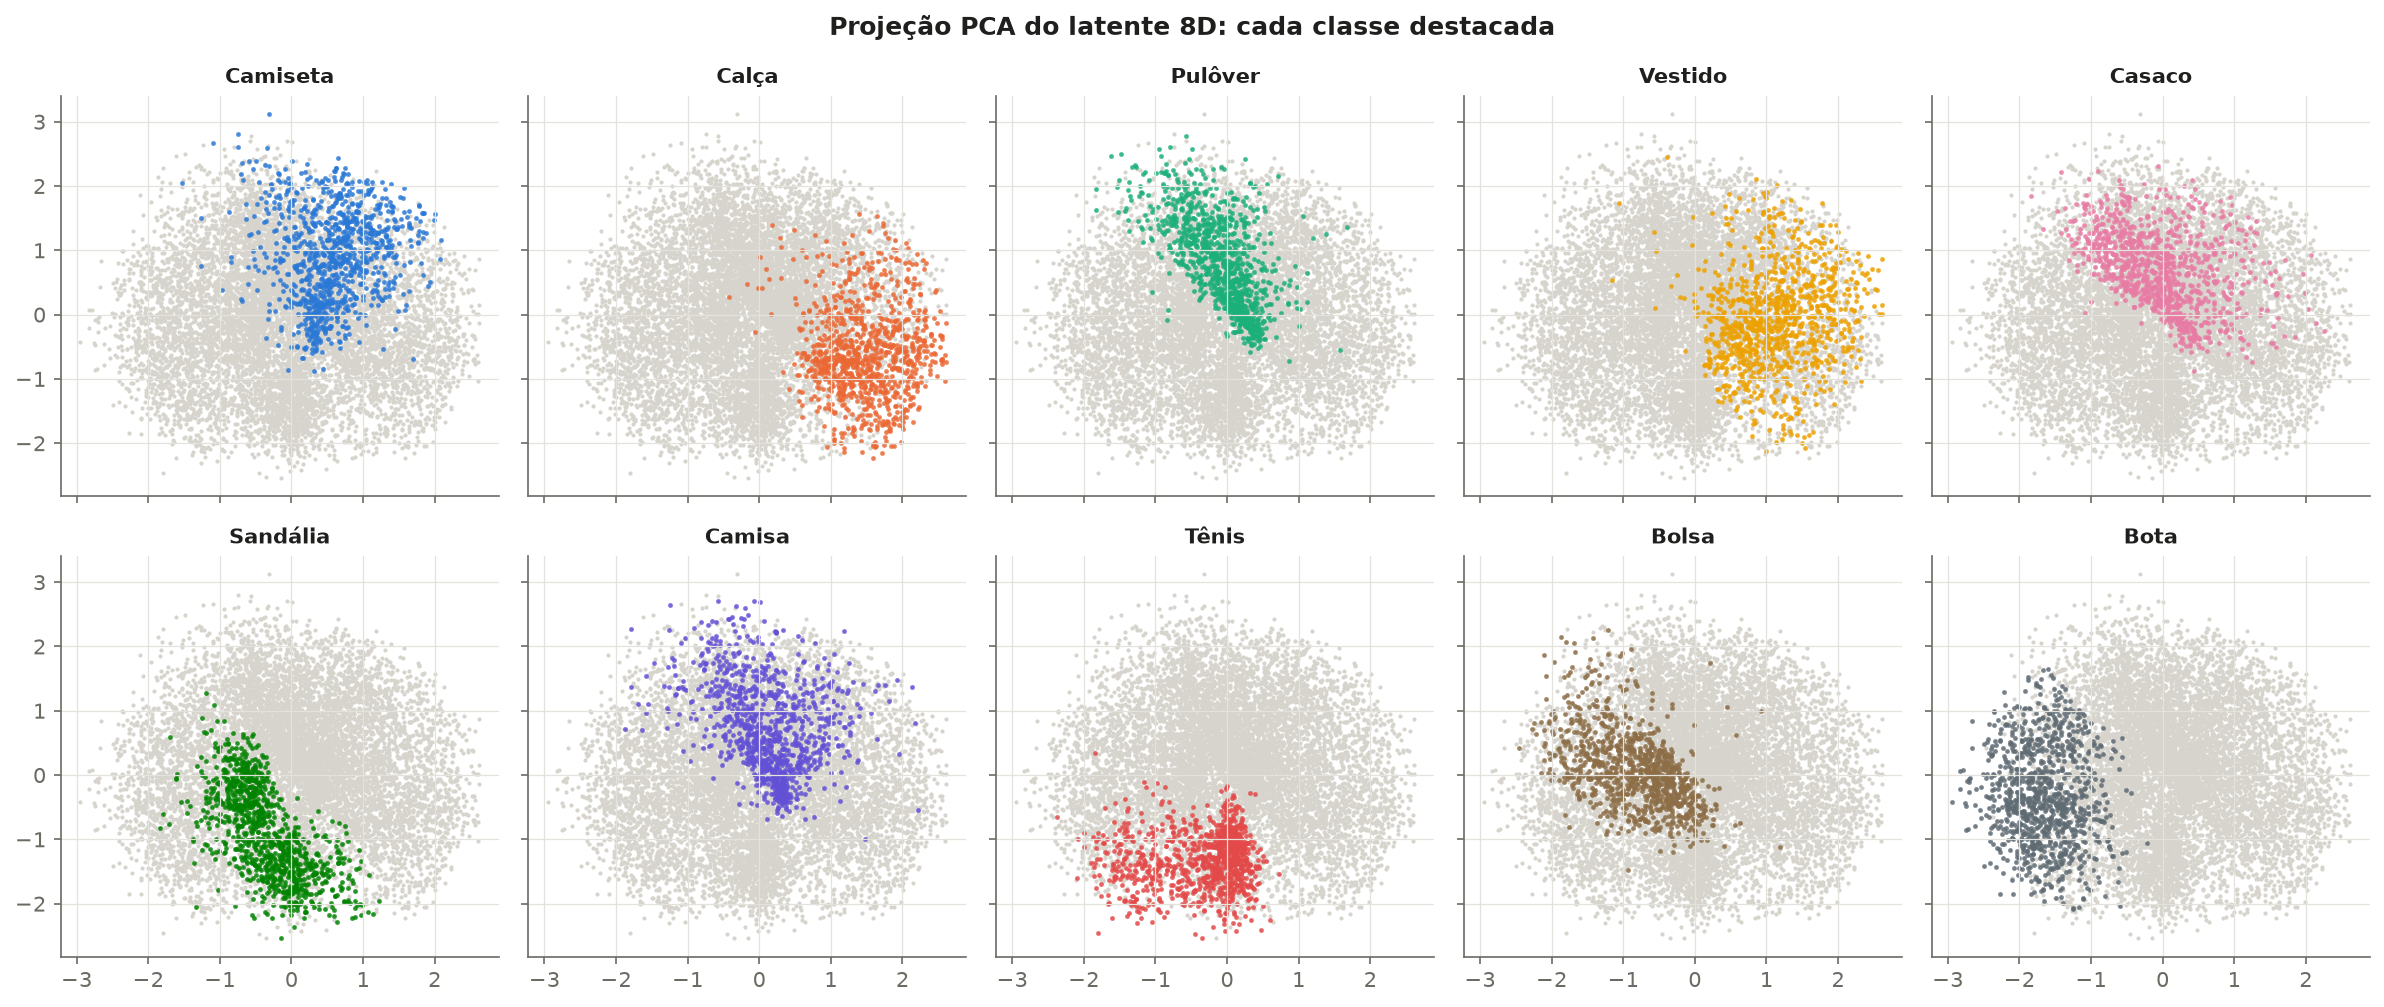
\includegraphics[width=\textwidth]{figs/pca_8d_por_classe.png}
    \caption{Projeção PCA do espaço latente 8D com cada classe destacada sobre as
    demais.}
    \label{fig:pca8d-classe}
\end{figure}

A projeção perde parte da separação existente no espaço completo. O coeficiente
de silhueta médio foi de $0{,}059$ no espaço 8D e caiu para $-0{,}002$ na
projeção, e na projeção as classes se sobrepõem mais do que no espaço latente 2D
treinado diretamente (silhueta de $0{,}056$). Parte da distinção entre as
classes está, portanto, nas componentes que a projeção descarta.

% =====================================================================
\section{Resultados e Discussão}

A respeito da formação de \emph{clusters} no espaço latente, observou-se que
eles não ocorrem na forma de grupos isolados. Nos dois espaços, as representações formam uma nuvem contínua em torno
da origem, e o coeficiente de silhueta ficou próximo de zero ($0{,}056$ no 2D e
$0{,}059$ no 8D). O que se observa são regiões mais densas e grupos de classes
vizinhas. Esse resultado é coerente com o funcionamento do VAE: o termo KL
aproxima as distribuições de todas as imagens da mesma normal padrão, o que as
faz se sobrepor e elimina os espaços vazios. É essa mesma propriedade que permite
gerar imagens a partir de qualquer ponto e obter transições suaves entre peças.
 
Em relação à separação dos rótulos no espaço latente, observou-se que ela
ocorre parcialmente, e de acordo com a semelhança visual. Os calçados, a calça e a bolsa ocupam regiões próprias,
enquanto camiseta, pulôver, casaco e camisa se sobrepõem, com a camisa com
silhueta negativa nas três representações. O espaço latente foi organizado
sem acesso aos rótulos e, por isso, reflete a aparência das imagens e não a
divisão em classes: peças parecidas ficam próximas mesmo quando têm rótulos
diferentes, e uma classe com estilos visualmente distintos, como a bolsa, pode ser
dividida. O coeficiente de silhueta deve ser lido com essa ressalva, pois
penaliza tanto classes encostadas quanto classes divididas em subgrupos.
 
Quanto à variância ilustrada pela projeção, observou-se que o espaço 8D
projetado nas duas primeiras componentes principais representa $45{,}6\%$ da
variância total. O valor é baixo
porque o modelo distribuiu a informação de forma quase uniforme entre as cinco
dimensões que usou, e porque o termo KL tende a igualar a variância das
dimensões. A projeção mostra os mesmos grupos de vizinhança do espaço 2D, mas
com mais sobreposição.
 
Os resultados devem ser lidos com algumas ressalvas. Cada modelo foi treinado uma
única vez, com semente fixa, e os hiperparâmetros não foram variados, então a
diferença entre a MLP profunda e a rede convolucional pode não se repetir. Os
modelos escolhidos também atingiram o limite de épocas. Em conclusão, os VAEs
aprenderam espaços latentes contínuos e organizados por semelhança visual, capazes
de gerar peças reconhecíveis. O espaço 2D permite visualização direta e
interpretação do mapa gerativo, mas força mais sobreposição; o espaço 8D
reconstrói melhor, mas só pode ser visto por uma projeção que mostra menos da
metade da sua variância.

% \textbf{Há formação de clusters no espaço latente?} Não na forma de grupos
% isolados. Nos dois espaços, as representações formam uma nuvem contínua em torno
% da origem, e o coeficiente de silhueta ficou próximo de zero ($0{,}056$ no 2D e
% $0{,}059$ no 8D). O que se observa são regiões mais densas e grupos de classes
% vizinhas. Esse resultado é coerente com o funcionamento do VAE: o termo KL
% aproxima as distribuições de todas as imagens da mesma normal padrão, o que as
% faz se sobrepor e elimina os espaços vazios. É essa mesma propriedade que permite
% gerar imagens a partir de qualquer ponto e obter transições suaves entre peças.

% \textbf{Há separação dos rótulos no espaço latente?} Parcialmente, e de acordo
% com a semelhança visual. Os calçados, a calça e a bolsa ocupam regiões próprias,
% enquanto camiseta, pulôver, casaco e camisa se sobrepõem, com a camisa com
% silhueta negativa nas três representações. O espaço latente foi organizado
% sem acesso aos rótulos e, por isso, reflete a aparência das imagens e não a
% divisão em classes: peças parecidas ficam próximas mesmo quando têm rótulos
% diferentes, e uma classe com estilos visualmente distintos, como a bolsa, pode ser
% dividida. O coeficiente de silhueta deve ser lido com essa ressalva, pois
% penaliza tanto classes encostadas quanto classes divididas em subgrupos.

% \textbf{A projeção ilustra quanto da variância?} A projeção do espaço 8D nas duas
% primeiras componentes principais ilustra $45{,}6\%$ da variância. O valor é baixo
% porque o modelo distribuiu a informação de forma quase uniforme entre as cinco
% dimensões que usou, e porque o termo KL tende a igualar a variância das
% dimensões. A projeção mostra os mesmos grupos de vizinhança do espaço 2D, mas
% com mais sobreposição.

% Os resultados devem ser lidos com algumas ressalvas. Cada modelo foi treinado uma
% única vez, com semente fixa, e os hiperparâmetros não foram variados, então a
% diferença entre a MLP profunda e a rede convolucional pode não se repetir. Os
% modelos escolhidos também atingiram o limite de épocas. Em conclusão, os VAEs
% aprenderam espaços latentes contínuos e organizados por semelhança visual, capazes
% de gerar peças reconhecíveis. O espaço 2D permite visualização direta e
% interpretação do mapa gerativo, mas força mais sobreposição; o espaço 8D
% reconstrói melhor, mas só pode ser visto por uma projeção que mostra menos da
% metade da sua variância.

\end{document}